\documentclass[11pt,a4paper]{ivoa}
\input tthdefs

\title{VOTable Format Definition}

% see ivoatexDoc for what group names to use here
\ivoagroup{Applications}

\author[http://www.ivoa.net/twiki/bin/view/IVOA/FrancoisOchsenbein]
                                               {Fran\c{c}ois Ochsenbein}
\author[http://www.ivoa.net/twiki/bin/view/IVOA/RoyWilliams]{Roy Williams}
\author[http://www.ivoa.net/twiki/bin/view/IVOA/CliveDavenhall]{Clive Davenhall}
\author[http://www.ivoa.net/twiki/bin/view/IVOA/MarkusDemleitner]
                                               {Markus Demleitner}
\author[http://www.ivoa.net/twiki/bin/view/IVOA/TomDonaldson]{Tom Donaldson}
\author[http://www.ivoa.net/twiki/bin/view/IVOA/DanielDurand]{Daniel Durand}
\author[http://www.ivoa.net/twiki/bin/view/IVOA/PierreFernique]{Pierre Fernique}
\author[http://www.ivoa.net/twiki/bin/view/IVOA/DavidGiaretta]{David Giaretta}
\author[http://www.ivoa.net/twiki/bin/view/IVOA/BobHanisch]{Robert Hanisch}
\author[http://www.ivoa.net/twiki/bin/view/IVOA/TomMcGlynn]{Tom McGlynn}
\author[http://www.ivoa.net/twiki/bin/view/IVOA/AlexSzalay]{Alex Szalay}
\author[http://www.ivoa.net/twiki/bin/view/IVOA/MarkTaylor]{Mark Taylor}
\author[http://www.ivoa.net/twiki/bin/view/IVOA/AndreasWicenec]{Andreas Wicenec}

\editor[http://www.ivoa.net/twiki/bin/view/IVOA/FrancoisOchsenbein]
                                               {Fran\c{c}ois Ochsenbein}
\editor[http://www.ivoa.net/twiki/bin/view/IVOA/MarkTaylor]{Mark Taylor}
\editor[http://www.ivoa.net/twiki/bin/view/IVOA/TomDonaldson]{Tom Donaldson}

\previousversion[http://www.ivoa.net/documents/VOTable/20130920/]
                {http://www.ivoa.net/documents/VOTable/20130920/
                 (V1.3 2013-09-20)}
\previousversion[http://www.ivoa.net/documents/VOTable/20091130/]
                {http://www.ivoa.net/documents/VOTable/20091130/
                 (V1.2 2009-11-30)}
\previousversion[http://www.ivoa.net/documents/cover/VOT-20040811.html]
                {http://www.ivoa.net/documents/cover/VOT-20040811.html
                 (V1.1 2004-08-11)}
\previousversion[http://www.ivoa.net/documents/PR/VOTable/VOTable-20031017.html]
                {http://www.ivoa.net/documents/PR/VOTable/VOTable-20031017.html
                 (V1.0 2003-10-17)}

\begin{document}
\begin{abstract}
This document describes the structures making up
the VOTable standard.

The main part of this document describes the adopted part of the
VOTable standard; it is followed by appendices presenting extensions
which have been proposed and/or discussed, but which are not part of
the standard.
\end{abstract}


% This section not included in REC-VOTable-1.4
% Possibly should be introduced into later versions for conformity
% with other IVOA docs; but the content would have to be reviewed
% to determine whether these terms actually are used like this.
%
% \section*{Conformance-related definitions}
% 
% The words ``MUST'', ``SHALL'', ``SHOULD'', ``MAY'', ``RECOMMENDED'', and
% ``OPTIONAL'' (in upper or lower case) used in this document are to be
% interpreted as described in IETF standard RFC2119 \citep{std:RFC2119}.
% 
% The \emph{Virtual Observatory (VO)} is a
% general term for a collection of federated resources that can be used
% to conduct astronomical research, education, and outreach.
% The \href{http://www.ivoa.net}{International
% Virtual Observatory Alliance (IVOA)} is a global
% collaboration of separately funded projects to develop standards and
% infrastructure that enable VO applications.


\section{Introduction}

???? Write something ????

\subsection{Role within the VO Architecture}

\begin{figure}
\centering

% As of ivoatex 1.2, the architecture diagram is generated by ivoatex in
% SVG; copy ivoatex/archdiag-full.xml to archdiag.xml and throw out
% all lines not relevant to your standard.
% Notes don't generally need this.  If you don't copy archdiag.xml,
% you must remove archdiag.svg from FIGURES in the Makefile.

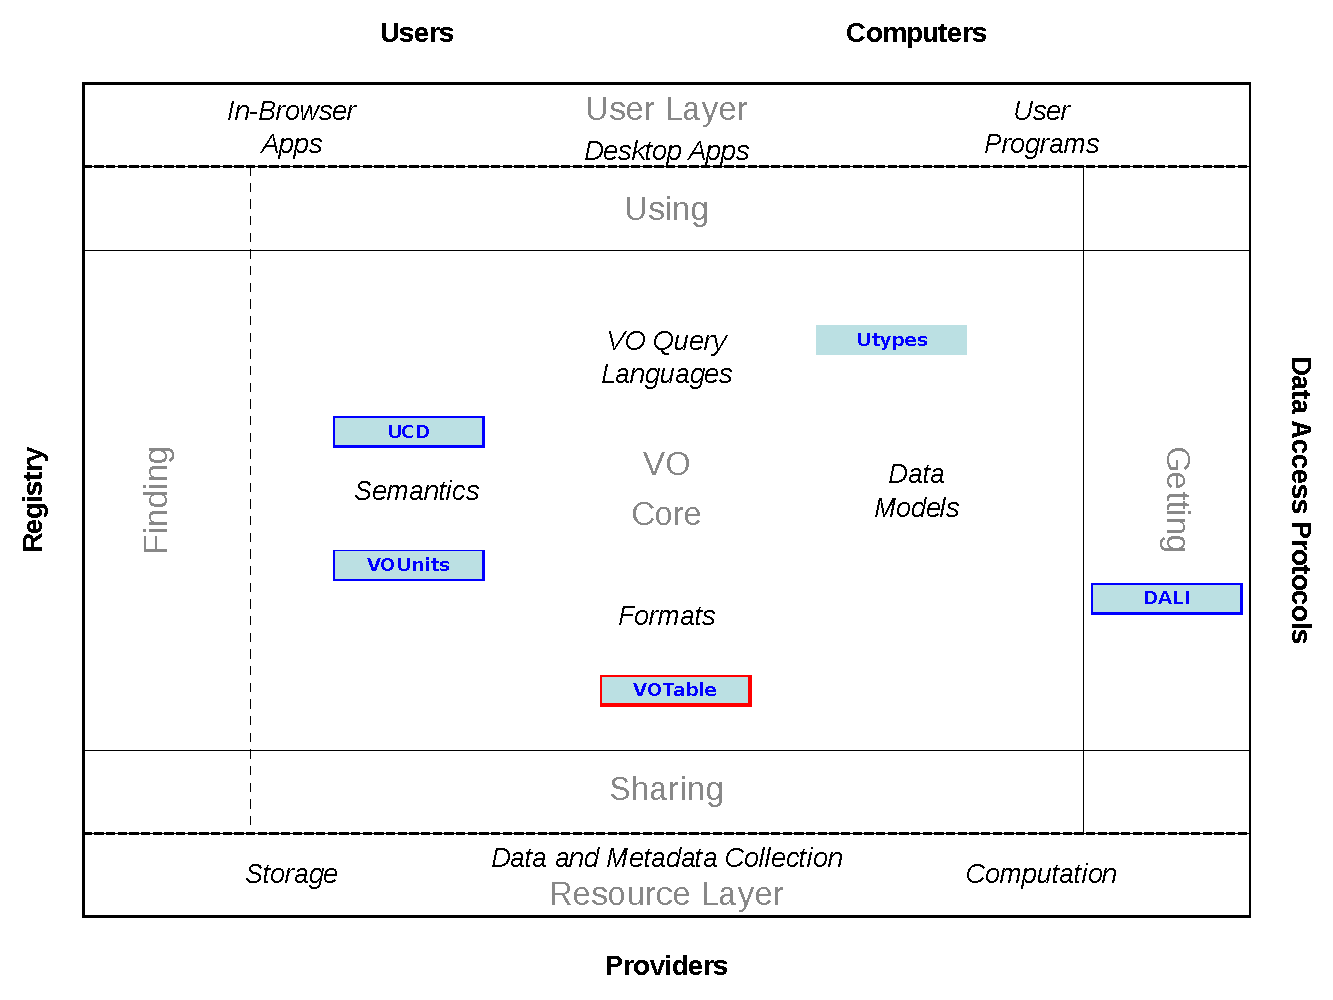
\includegraphics[width=0.9\textwidth]{role_diagram.pdf}
\caption{Architecture diagram for this document}
\label{fig:archdiag}
\end{figure}

Fig.~\ref{fig:archdiag} shows the role this document plays within the
IVOA architecture \citep{note:VOARCH}.

???? and so on, LaTeX as you know and love it. ????

\appendix
\section{Changes from Previous Versions}

% these would be subsections "Changes from v. WD-..."
% Use itemize environments.


% NOTE: IVOA recommendations must be cited from docrepo rather than ivoabib
% (REC entries there are for legacy documents only)
\bibliography{ivoatex/ivoabib,ivoatex/docrepo}


\end{document}
